\documentclass[aspectratio=169]{beamer}

\usepackage[utf8]{inputenc}
\usepackage{lmodern}
\usepackage[T1]{fontenc}
\usepackage{amsmath}
\usepackage{listings}
\usepackage{xcolor}
\usepackage{graphicx}
\usepackage{tikz}
\usetikzlibrary{arrows.meta, positioning, shapes.geometric, calc, trees, shapes.multipart}

\makeatletter
\def\input@path{{../BeamerTemplate/theme/}}
\makeatother

\usetheme{CleanEasy}

\input{../BeamerTemplate/configs/configs}

\title{Trees}
\subtitle{Hierarchical Data Structures}
\author{Minseok Jeon}
\institute{DGIST}
\date{\today}

\begin{document}

\begin{frame}
  \titlepage
\end{frame}

\begin{frame}{Outline}
  \tableofcontents
\end{frame}

\section{Introduction to Trees}

\begin{frame}{What is a Tree?}
  \textbf{Definition:} A hierarchical data structure consisting of nodes connected by edges.

  \vspace{0.3cm}
  \textbf{Key Properties:}
  \begin{itemize}
    \item Exactly one path between any two nodes
    \item One designated \textbf{root} node at the top
    \item No cycles (acyclic graph)
    \item Each node has zero or more \textbf{children}
  \end{itemize}

  \vspace{0.3cm}
  \textbf{Tree Terminology:}
  \begin{itemize}
    \item \textbf{Root:} The topmost node
    \item \textbf{Parent:} A node that has children
    \item \textbf{Child:} A node connected to a parent
    \item \textbf{Leaf:} A node with no children
    \item \textbf{Height:} Longest path from root to a leaf
    \item \textbf{Depth:} Distance from root to a node
  \end{itemize}
\end{frame}

\begin{frame}{Basic Tree Structure}
  \begin{center}
    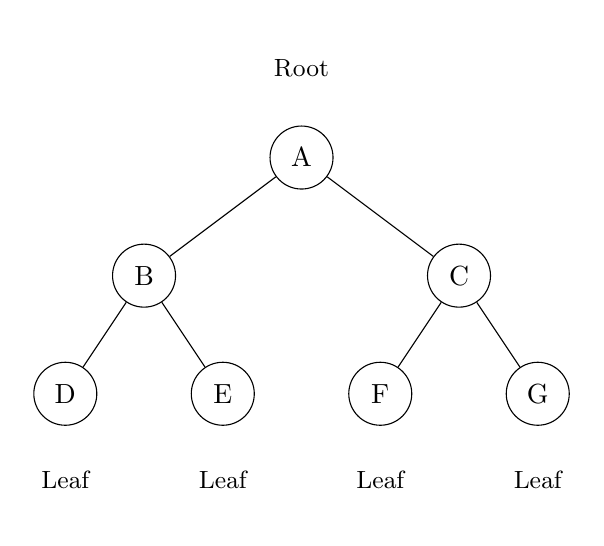
\begin{tikzpicture}[
      level distance=1.5cm,
      level 1/.style={sibling distance=4cm},
      level 2/.style={sibling distance=2cm},
      every node/.style={circle, draw, minimum size=0.8cm}
    ]
      \node (A) {A}
        child {node (B) {B}
          child {node (D) {D}}
          child {node (E) {E}}
        }
        child {node (C) {C}
          child {node (F) {F}}
          child {node (G) {G}}
        };

      \node[above=0.2cm of A, draw=none] {\small Root};
      \node[below=0.2cm of D, draw=none] {\small Leaf};
      \node[below=0.2cm of E, draw=none] {\small Leaf};
      \node[below=0.2cm of F, draw=none] {\small Leaf};
      \node[below=0.2cm of G, draw=none] {\small Leaf};
    \end{tikzpicture}
  \end{center}

  \vspace{0.3cm}
  \begin{itemize}
    \item \textbf{Root:} A
    \item \textbf{Internal nodes:} B, C
    \item \textbf{Leaves:} D, E, F, G
    \item \textbf{Height:} 2
  \end{itemize}
\end{frame}

\begin{frame}{Why Use Trees?}
  \textbf{Advantages:}
  \begin{itemize}
    \item \textbf{Natural hierarchy:} File systems, organizational charts
    \item \textbf{Efficient search:} O(log n) in balanced trees
    \item \textbf{Fast insertion/deletion:} Compared to sorted arrays
    \item \textbf{Flexible structure:} Adapts to different data patterns
  \end{itemize}

  \vspace{0.3cm}
  \textbf{Common Applications:}
  \begin{itemize}
    \item Database indexing (B-trees)
    \item File systems (directory trees)
    \item Expression parsing (syntax trees)
    \item Decision making (decision trees)
    \item Network routing
    \item Compression algorithms (Huffman trees)
  \end{itemize}
\end{frame}

\section{Binary Trees}

\begin{frame}{Binary Trees}
  \textbf{Definition:} A tree where each node has at most two children (left and right).

  \vspace{0.3cm}
  \begin{center}
    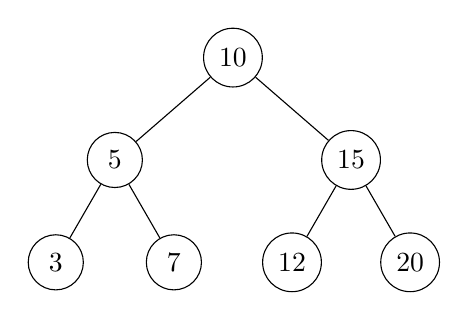
\begin{tikzpicture}[
      level distance=1.3cm,
      level 1/.style={sibling distance=3cm},
      level 2/.style={sibling distance=1.5cm},
      every node/.style={circle, draw, minimum size=0.7cm}
    ]
      \node {10}
        child {node {5}
          child {node {3}}
          child {node {7}}
        }
        child {node {15}
          child {node {12}}
          child {node {20}}
        };
    \end{tikzpicture}
  \end{center}

  \vspace{0.3cm}
  \textbf{Properties:}
  \begin{itemize}
    \item Each node: at most 2 children
    \item Left child $<$ Parent (in BST)
    \item Right child $>$ Parent (in BST)
  \end{itemize}
\end{frame}

\begin{frame}{Types of Binary Trees: Full Binary Tree}
  \textbf{Full Binary Tree:} Every node has either 0 or 2 children (no nodes with 1 child).

  \vspace{0.3cm}
  \begin{center}
    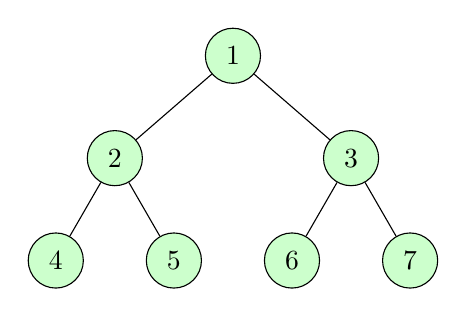
\begin{tikzpicture}[
      level distance=1.3cm,
      level 1/.style={sibling distance=3cm},
      level 2/.style={sibling distance=1.5cm},
      every node/.style={circle, draw, minimum size=0.7cm, fill=green!20}
    ]
      \node {1}
        child {node {2}
          child {node {4}}
          child {node {5}}
        }
        child {node {3}
          child {node {6}}
          child {node {7}}
        };
    \end{tikzpicture}
  \end{center}

  \vspace{0.3cm}
  \textbf{Characteristics:}
  \begin{itemize}
    \item All internal nodes have exactly 2 children
    \item All leaves at same or adjacent levels
    \item Useful for expression trees
  \end{itemize}
\end{frame}

\begin{frame}{Types of Binary Trees: Complete Binary Tree}
  \textbf{Complete Binary Tree:} All levels filled except possibly the last, which is filled from left to right.

  \vspace{0.3cm}
  \begin{center}
    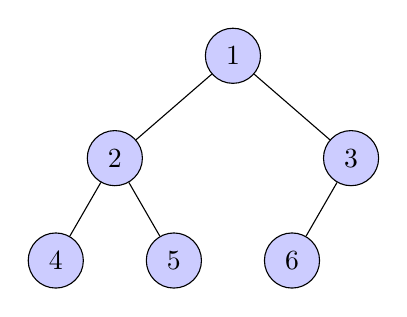
\begin{tikzpicture}[
      level distance=1.3cm,
      level 1/.style={sibling distance=3cm},
      level 2/.style={sibling distance=1.5cm},
      every node/.style={circle, draw, minimum size=0.7cm, fill=blue!20}
    ]
      \node {1}
        child {node {2}
          child {node {4}}
          child {node {5}}
        }
        child {node {3}
          child {node {6}}
          child[missing] {}
        };
    \end{tikzpicture}
  \end{center}

  \vspace{0.3cm}
  \textbf{Characteristics:}
  \begin{itemize}
    \item Used in heap data structures
    \item Can be efficiently stored in arrays
    \item Left-to-right filling at each level
  \end{itemize}
\end{frame}

\begin{frame}{Types of Binary Trees: Perfect Binary Tree}
  \textbf{Perfect Binary Tree:} All internal nodes have 2 children and all leaves are at the same level.

  \vspace{0.3cm}
  \begin{center}
    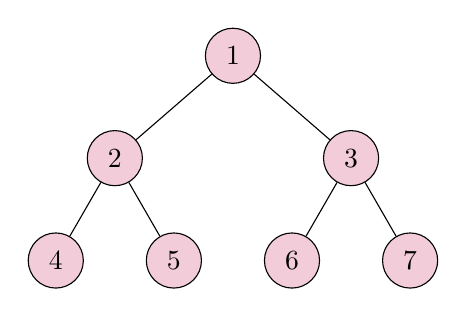
\begin{tikzpicture}[
      level distance=1.3cm,
      level 1/.style={sibling distance=3cm},
      level 2/.style={sibling distance=1.5cm},
      every node/.style={circle, draw, minimum size=0.7cm, fill=purple!20}
    ]
      \node {1}
        child {node {2}
          child {node {4}}
          child {node {5}}
        }
        child {node {3}
          child {node {6}}
          child {node {7}}
        };
    \end{tikzpicture}
  \end{center}

  \vspace{0.3cm}
  \textbf{Properties:}
  \begin{itemize}
    \item Total nodes = $2^{h+1} - 1$ (h = height)
    \item All leaves at level h
    \item Maximally space-efficient
  \end{itemize}
\end{frame}

\begin{frame}{Types of Binary Trees: Balanced vs Skewed}
  \begin{columns}[T]
    \begin{column}{0.5\textwidth}
      \textbf{Balanced Binary Tree}

      Height difference $\leq$ 1 for all nodes

      \vspace{0.2cm}
      \begin{center}
        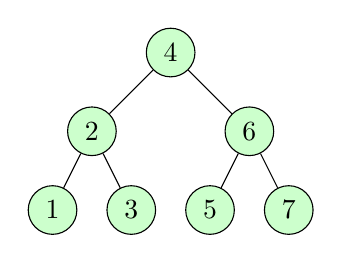
\begin{tikzpicture}[
          level distance=1cm,
          level 1/.style={sibling distance=2cm},
          level 2/.style={sibling distance=1cm},
          every node/.style={circle, draw, minimum size=0.6cm, fill=green!20}
        ]
          \node {4}
            child {node {2}
              child {node {1}}
              child {node {3}}
            }
            child {node {6}
              child {node {5}}
              child {node {7}}
            };
        \end{tikzpicture}
      \end{center}

      \textbf{Height:} O(log n)
    \end{column}

    \begin{column}{0.5\textwidth}
      \textbf{Skewed Binary Tree}

      All nodes only have one child

      \vspace{0.2cm}
      \begin{center}
        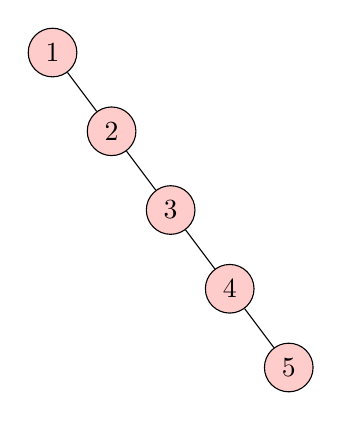
\begin{tikzpicture}[
          level distance=1cm,
          every node/.style={circle, draw, minimum size=0.6cm, fill=red!20}
        ]
          \node {1}
            child[missing] {}
            child {node {2}
              child[missing] {}
              child {node {3}
                child[missing] {}
                child {node {4}
                  child[missing] {}
                  child {node {5}}
                }
              }
            };
        \end{tikzpicture}
      \end{center}

      \textbf{Height:} O(n)
    \end{column}
  \end{columns}
\end{frame}

\begin{frame}[fragile]{Binary Tree Implementation}
  \begin{lstlisting}[language=Python, basicstyle=\ttfamily\small]
class TreeNode:
    def __init__(self, value):
        self.value = value
        self.left = None
        self.right = None

class BinaryTree:
    def __init__(self):
        self.root = None

    def insert(self, value):
        if not self.root:
            self.root = TreeNode(value)
        else:
            self._insert_recursive(self.root, value)

    def _insert_recursive(self, node, value):
        if value < node.value:
            if node.left is None:
                node.left = TreeNode(value)
            else:
                self._insert_recursive(node.left, value)
        else:
            if node.right is None:
                node.right = TreeNode(value)
            else:
                self._insert_recursive(node.right, value)
  \end{lstlisting}
\end{frame}

\section{Binary Search Trees (BST)}

\begin{frame}{Binary Search Tree (BST)}
  \textbf{Definition:} A binary tree where for every node:
  \begin{itemize}
    \item All values in left subtree $<$ node value
    \item All values in right subtree $>$ node value
    \item Both subtrees are also BSTs
  \end{itemize}

  \vspace{0.3cm}
  \begin{center}
    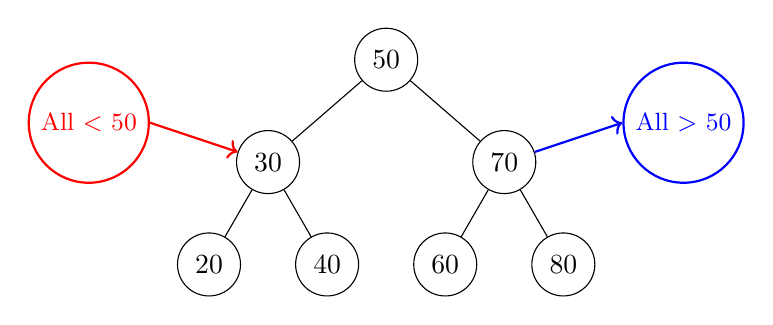
\begin{tikzpicture}[
      level distance=1.3cm,
      level 1/.style={sibling distance=3cm},
      level 2/.style={sibling distance=1.5cm},
      every node/.style={circle, draw, minimum size=0.8cm}
    ]
      \node (n50) {50}
        child {node (n30) {30}
          child {node {20}}
          child {node {40}}
        }
        child {node (n70) {70}
          child {node {60}}
          child {node {80}}
        };

      \draw[<-, thick, red] (n30) -- ++(-1.5, 0.5) node[left] {\small All $<$ 50};
      \draw[->, thick, blue] (n70) -- ++(1.5, 0.5) node[right] {\small All $>$ 50};
    \end{tikzpicture}
  \end{center}
\end{frame}

\begin{frame}{BST Search Operation}
  \textbf{Algorithm:} Start at root and compare target with current node.

  \vspace{0.3cm}
  \begin{center}
    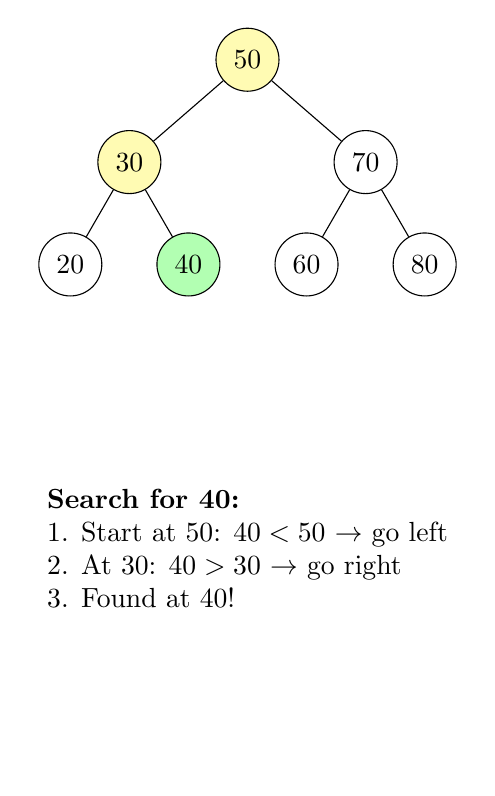
\begin{tikzpicture}[
      level distance=1.3cm,
      level 1/.style={sibling distance=3cm},
      level 2/.style={sibling distance=1.5cm},
      every node/.style={circle, draw, minimum size=0.8cm}
    ]
      \node[fill=yellow!30] (s50) {50}
        child {node[fill=yellow!30] {30}
          child {node {20}}
          child {node[fill=green!30] {40}}
        }
        child {node {70}
          child {node {60}}
          child {node {80}}
        };

      \node[below=3cm of s50, draw=none, align=left] {
        \textbf{Search for 40:}\\
        1. Start at 50: $40 < 50$ $\rightarrow$ go left\\
        2. At 30: $40 > 30$ $\rightarrow$ go right\\
        3. Found at 40!
      };
    \end{tikzpicture}
  \end{center}

  \textbf{Time Complexity:} O(h) where h is height
  \begin{itemize}
    \item Best case (balanced): O(log n)
    \item Worst case (skewed): O(n)
  \end{itemize}
\end{frame}

\begin{frame}[fragile]{BST Search Implementation}
  \begin{lstlisting}[language=Python, basicstyle=\ttfamily\small]
def search(self, value):
    """Search for a value in the BST"""
    return self._search_recursive(self.root, value)

def _search_recursive(self, node, value):
    # Base case: empty tree or value found
    if node is None or node.value == value:
        return node

    # Value is smaller: search left subtree
    if value < node.value:
        return self._search_recursive(node.left, value)

    # Value is larger: search right subtree
    return self._search_recursive(node.right, value)

# Iterative version
def search_iterative(self, value):
    current = self.root
    while current:
        if value == current.value:
            return current
        elif value < current.value:
            current = current.left
        else:
            current = current.right
    return None
  \end{lstlisting}
\end{frame}

\begin{frame}[fragile]{BST Insert Operation}
  \begin{lstlisting}[language=Python, basicstyle=\ttfamily\small]
def insert(self, value):
    """Insert a value into the BST"""
    if not self.root:
        self.root = TreeNode(value)
    else:
        self._insert_recursive(self.root, value)

def _insert_recursive(self, node, value):
    # Insert in left subtree
    if value < node.value:
        if node.left is None:
            node.left = TreeNode(value)
        else:
            self._insert_recursive(node.left, value)
    # Insert in right subtree
    else:
        if node.right is None:
            node.right = TreeNode(value)
        else:
            self._insert_recursive(node.right, value)
  \end{lstlisting}

  \vspace{0.3cm}
  \textbf{Time Complexity:} O(h) where h is height
\end{frame}

\begin{frame}{BST Delete Operation: Three Cases}
  \textbf{Case 1: Node is a leaf} $\rightarrow$ Simply remove it

  \textbf{Case 2: Node has one child} $\rightarrow$ Replace with child

  \textbf{Case 3: Node has two children} $\rightarrow$ Replace with:
  \begin{itemize}
    \item \textbf{Inorder successor:} Smallest value in right subtree
    \item \textbf{Inorder predecessor:} Largest value in left subtree
  \end{itemize}

  \vspace{0.3cm}
  \begin{center}
    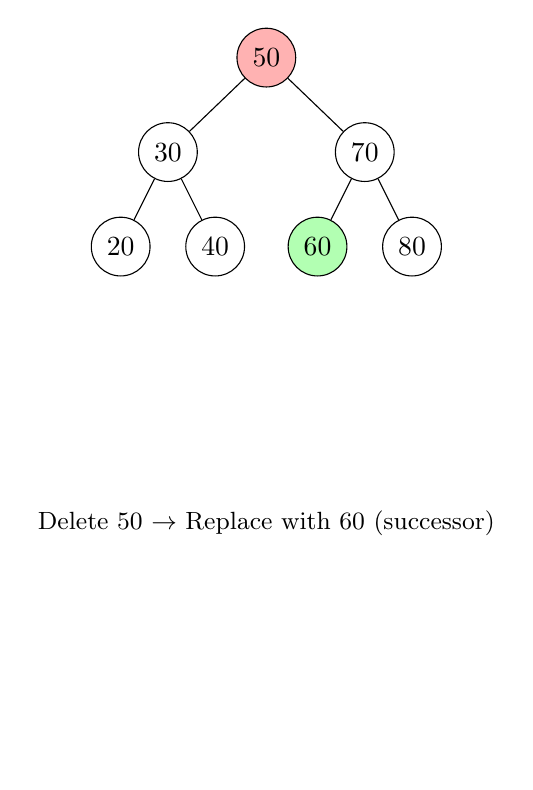
\begin{tikzpicture}[
      level distance=1.2cm,
      level 1/.style={sibling distance=2.5cm},
      level 2/.style={sibling distance=1.2cm},
      every node/.style={circle, draw, minimum size=0.7cm}
    ]
      \node[fill=red!30] (d50) {50}
        child {node {30}
          child {node {20}}
          child {node {40}}
        }
        child {node {70}
          child {node[fill=green!30] {60}}
          child {node {80}}
        };

      \node[below=2.5cm of d50, draw=none] {\small Delete 50 $\rightarrow$ Replace with 60 (successor)};
    \end{tikzpicture}
  \end{center}
\end{frame}

\begin{frame}[fragile]{BST Delete Implementation}
  \begin{lstlisting}[language=Python, basicstyle=\ttfamily\footnotesize]
def delete(self, value):
    self.root = self._delete_recursive(self.root, value)

def _delete_recursive(self, node, value):
    if node is None:
        return None

    if value < node.value:
        node.left = self._delete_recursive(node.left, value)
    elif value > node.value:
        node.right = self._delete_recursive(node.right, value)
    else:
        # Case 1: Leaf or one child
        if node.left is None:
            return node.right
        if node.right is None:
            return node.left

        # Case 2: Two children - find inorder successor
        successor = self._find_min(node.right)
        node.value = successor.value
        node.right = self._delete_recursive(node.right, successor.value)

    return node

def _find_min(self, node):
    while node.left:
        node = node.left
    return node
  \end{lstlisting}
\end{frame}

\section{Tree Traversals}

\begin{frame}{Tree Traversal Overview}
  \textbf{Traversal:} Visiting all nodes in a specific order.

  \vspace{0.3cm}
  \textbf{Four Main Types:}
  \begin{enumerate}
    \item \textbf{Inorder (Left-Root-Right):} Produces sorted order in BST
    \item \textbf{Preorder (Root-Left-Right):} Used for copying trees
    \item \textbf{Postorder (Left-Right-Root):} Used for deleting trees
    \item \textbf{Level-order (Breadth-first):} Level by level
  \end{enumerate}

  \vspace{0.3cm}
  \begin{center}
    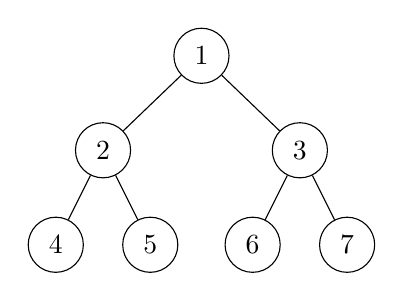
\begin{tikzpicture}[
      level distance=1.2cm,
      level 1/.style={sibling distance=2.5cm},
      level 2/.style={sibling distance=1.2cm},
      every node/.style={circle, draw, minimum size=0.7cm}
    ]
      \node {1}
        child {node {2}
          child {node {4}}
          child {node {5}}
        }
        child {node {3}
          child {node {6}}
          child {node {7}}
        };
    \end{tikzpicture}
  \end{center}
\end{frame}

\begin{frame}{Inorder Traversal (Left-Root-Right)}
  \textbf{Order:} Left subtree $\rightarrow$ Root $\rightarrow$ Right subtree

  \vspace{0.3cm}
  \begin{center}
    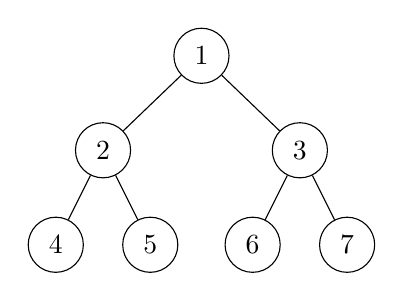
\begin{tikzpicture}[
      level distance=1.2cm,
      level 1/.style={sibling distance=2.5cm},
      level 2/.style={sibling distance=1.2cm},
      every node/.style={circle, draw, minimum size=0.7cm}
    ]
      \node {1}
        child {node {2}
          child {node {4}}
          child {node {5}}
        }
        child {node {3}
          child {node {6}}
          child {node {7}}
        };
    \end{tikzpicture}
  \end{center}

  \textbf{Result:} 4, 2, 5, 1, 6, 3, 7

  \vspace{0.3cm}
  \textbf{Use Cases:}
  \begin{itemize}
    \item Getting sorted order from BST
    \item Expression tree evaluation
  \end{itemize}
\end{frame}

\begin{frame}[fragile]{Inorder Traversal Implementation}
  \begin{lstlisting}[language=Python, basicstyle=\ttfamily\small]
def inorder(self):
    """Return list of values in inorder"""
    result = []
    self._inorder_recursive(self.root, result)
    return result

def _inorder_recursive(self, node, result):
    if node:
        # Left subtree
        self._inorder_recursive(node.left, result)
        # Root
        result.append(node.value)
        # Right subtree
        self._inorder_recursive(node.right, result)

# Iterative version using stack
def inorder_iterative(self):
    result, stack = [], []
    current = self.root
    while current or stack:
        while current:
            stack.append(current)
            current = current.left
        current = stack.pop()
        result.append(current.value)
        current = current.right
    return result
  \end{lstlisting}
\end{frame}

\begin{frame}{Preorder Traversal (Root-Left-Right)}
  \textbf{Order:} Root $\rightarrow$ Left subtree $\rightarrow$ Right subtree

  \vspace{0.3cm}
  \begin{center}
    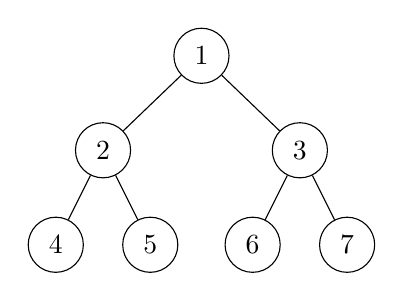
\begin{tikzpicture}[
      level distance=1.2cm,
      level 1/.style={sibling distance=2.5cm},
      level 2/.style={sibling distance=1.2cm},
      every node/.style={circle, draw, minimum size=0.7cm}
    ]
      \node {1}
        child {node {2}
          child {node {4}}
          child {node {5}}
        }
        child {node {3}
          child {node {6}}
          child {node {7}}
        };
    \end{tikzpicture}
  \end{center}

  \textbf{Result:} 1, 2, 4, 5, 3, 6, 7

  \vspace{0.3cm}
  \textbf{Use Cases:}
  \begin{itemize}
    \item Creating a copy of the tree
    \item Prefix expression of an expression tree
    \item Serializing a tree
  \end{itemize}
\end{frame}

\begin{frame}[fragile]{Preorder Traversal Implementation}
  \begin{lstlisting}[language=Python, basicstyle=\ttfamily\small]
def preorder(self):
    """Return list of values in preorder"""
    result = []
    self._preorder_recursive(self.root, result)
    return result

def _preorder_recursive(self, node, result):
    if node:
        # Root
        result.append(node.value)
        # Left subtree
        self._preorder_recursive(node.left, result)
        # Right subtree
        self._preorder_recursive(node.right, result)

# Iterative version
def preorder_iterative(self):
    if not self.root:
        return []
    result, stack = [], [self.root]
    while stack:
        node = stack.pop()
        result.append(node.value)
        if node.right:
            stack.append(node.right)
        if node.left:
            stack.append(node.left)
    return result
  \end{lstlisting}
\end{frame}

\begin{frame}{Postorder Traversal (Left-Right-Root)}
  \textbf{Order:} Left subtree $\rightarrow$ Right subtree $\rightarrow$ Root

  \vspace{0.3cm}
  \begin{center}
    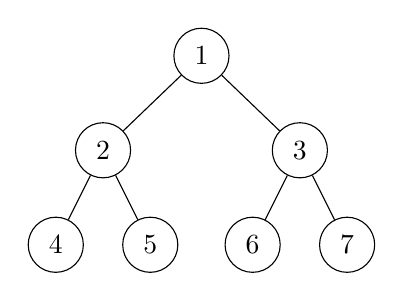
\begin{tikzpicture}[
      level distance=1.2cm,
      level 1/.style={sibling distance=2.5cm},
      level 2/.style={sibling distance=1.2cm},
      every node/.style={circle, draw, minimum size=0.7cm}
    ]
      \node {1}
        child {node {2}
          child {node {4}}
          child {node {5}}
        }
        child {node {3}
          child {node {6}}
          child {node {7}}
        };
    \end{tikzpicture}
  \end{center}

  \textbf{Result:} 4, 5, 2, 6, 7, 3, 1

  \vspace{0.3cm}
  \textbf{Use Cases:}
  \begin{itemize}
    \item Deleting a tree (delete children before parent)
    \item Postfix expression of an expression tree
    \item Computing directory sizes in file system
  \end{itemize}
\end{frame}

\begin{frame}[fragile]{Postorder Traversal Implementation}
  \begin{lstlisting}[language=Python, basicstyle=\ttfamily\small]
def postorder(self):
    """Return list of values in postorder"""
    result = []
    self._postorder_recursive(self.root, result)
    return result

def _postorder_recursive(self, node, result):
    if node:
        # Left subtree
        self._postorder_recursive(node.left, result)
        # Right subtree
        self._postorder_recursive(node.right, result)
        # Root
        result.append(node.value)

# Iterative version using two stacks
def postorder_iterative(self):
    if not self.root:
        return []
    stack1, stack2 = [self.root], []
    while stack1:
        node = stack1.pop()
        stack2.append(node)
        if node.left:
            stack1.append(node.left)
        if node.right:
            stack1.append(node.right)
    return [node.value for node in reversed(stack2)]
  \end{lstlisting}
\end{frame}

\begin{frame}{Level-Order Traversal (Breadth-First)}
  \textbf{Order:} Visit nodes level by level, left to right

  \vspace{0.3cm}
  \begin{center}
    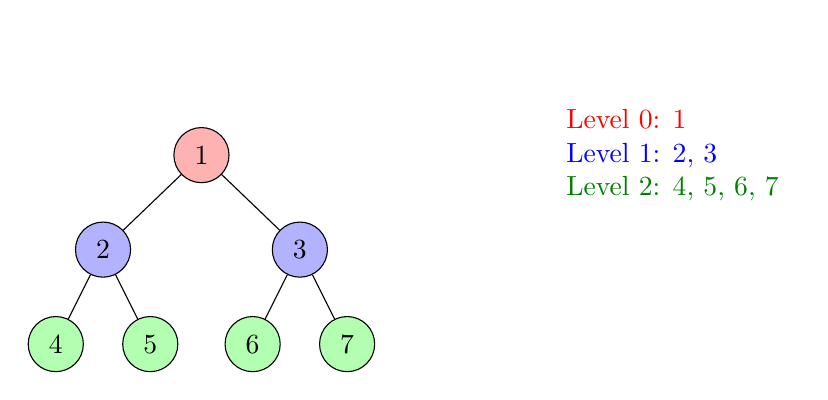
\begin{tikzpicture}[
      level distance=1.2cm,
      level 1/.style={sibling distance=2.5cm},
      level 2/.style={sibling distance=1.2cm},
      every node/.style={circle, draw, minimum size=0.7cm}
    ]
      \node[fill=red!30] (l1) {1}
        child {node[fill=blue!30] {2}
          child {node[fill=green!30] {4}}
          child {node[fill=green!30] {5}}
        }
        child {node[fill=blue!30] {3}
          child {node[fill=green!30] {6}}
          child {node[fill=green!30] {7}}
        };

      \node[right=4cm of l1, draw=none, align=left] {
        \textcolor{red}{Level 0: 1}\\
        \textcolor{blue}{Level 1: 2, 3}\\
        \textcolor{green!50!black}{Level 2: 4, 5, 6, 7}
      };
    \end{tikzpicture}
  \end{center}

  \textbf{Result:} 1, 2, 3, 4, 5, 6, 7

  \vspace{0.3cm}
  \textbf{Use Cases:}
  \begin{itemize}
    \item Finding shortest path in unweighted tree
    \item Level-wise processing
    \item Printing tree level by level
  \end{itemize}
\end{frame}

\begin{frame}[fragile]{Level-Order Traversal Implementation}
  \begin{lstlisting}[language=Python, basicstyle=\ttfamily\small]
from collections import deque

def level_order(self):
    """Return list of values in level-order"""
    if not self.root:
        return []

    result = []
    queue = deque([self.root])

    while queue:
        node = queue.popleft()
        result.append(node.value)

        if node.left:
            queue.append(node.left)
        if node.right:
            queue.append(node.right)

    return result

# Level-by-level (returns list of lists)
def level_order_levels(self):
    if not self.root:
        return []
    result, queue = [], deque([self.root])
    while queue:
        level = []
        for _ in range(len(queue)):
            node = queue.popleft()
            level.append(node.value)
            if node.left: queue.append(node.left)
            if node.right: queue.append(node.right)
        result.append(level)
    return result
  \end{lstlisting}
\end{frame}

\section{Heaps}

\begin{frame}{Heap Data Structure}
  \textbf{Definition:} A complete binary tree satisfying the heap property.

  \vspace{0.3cm}
  \textbf{Two Types:}
  \begin{itemize}
    \item \textbf{Max Heap:} Parent $\geq$ children (root is maximum)
    \item \textbf{Min Heap:} Parent $\leq$ children (root is minimum)
  \end{itemize}

  \vspace{0.3cm}
  \begin{columns}[T]
    \begin{column}{0.5\textwidth}
      \textbf{Max Heap}
      \begin{center}
        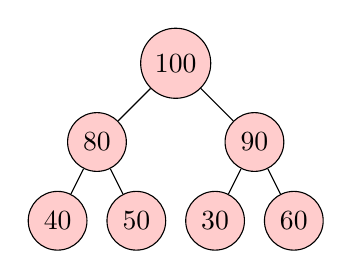
\begin{tikzpicture}[
          level distance=1cm,
          level 1/.style={sibling distance=2cm},
          level 2/.style={sibling distance=1cm},
          every node/.style={circle, draw, minimum size=0.6cm, fill=red!20}
        ]
          \node {100}
            child {node {80}
              child {node {40}}
              child {node {50}}
            }
            child {node {90}
              child {node {30}}
              child {node {60}}
            };
        \end{tikzpicture}
      \end{center}
    \end{column}

    \begin{column}{0.5\textwidth}
      \textbf{Min Heap}
      \begin{center}
        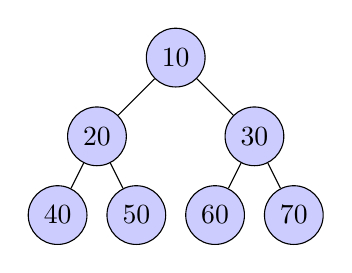
\begin{tikzpicture}[
          level distance=1cm,
          level 1/.style={sibling distance=2cm},
          level 2/.style={sibling distance=1cm},
          every node/.style={circle, draw, minimum size=0.6cm, fill=blue!20}
        ]
          \node {10}
            child {node {20}
              child {node {40}}
              child {node {50}}
            }
            child {node {30}
              child {node {60}}
              child {node {70}}
            };
        \end{tikzpicture}
      \end{center}
    \end{column}
  \end{columns}
\end{frame}

\begin{frame}{Heap Array Representation}
  \textbf{Key Insight:} Complete binary tree can be stored efficiently in an array.

  \vspace{0.3cm}
  \textbf{Index Relationships:}
  \begin{itemize}
    \item \textbf{Parent of i:} $(i-1) / 2$
    \item \textbf{Left child of i:} $2i + 1$
    \item \textbf{Right child of i:} $2i + 2$
  \end{itemize}

  \vspace{0.3cm}
  \begin{center}
    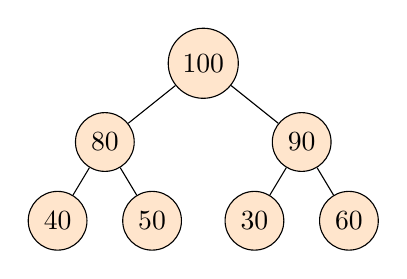
\begin{tikzpicture}[
      level distance=1cm,
      level 1/.style={sibling distance=2.5cm},
      level 2/.style={sibling distance=1.2cm},
      every node/.style={circle, draw, minimum size=0.7cm, fill=orange!20}
    ]
      \node {100}
        child {node {80}
          child {node {40}}
          child {node {50}}
        }
        child {node {90}
          child {node {30}}
          child {node {60}}
        };
    \end{tikzpicture}
  \end{center}

  \vspace{0.3cm}
  \textbf{Array:} [100, 80, 90, 40, 50, 30, 60]

  \textbf{Indices:} \quad 0 \quad 1 \quad 2 \quad 3 \quad 4 \quad 5 \quad 6
\end{frame}

\begin{frame}[fragile]{Heap Insert Operation}
  \textbf{Algorithm:}
  \begin{enumerate}
    \item Add new element at the end (maintain complete tree property)
    \item \textbf{Heapify Up:} Compare with parent and swap if needed
    \item Repeat until heap property restored
  \end{enumerate}

  \vspace{0.3cm}
  \begin{lstlisting}[language=Python, basicstyle=\ttfamily\small]
def insert(self, value):
    """Insert value into max heap"""
    self.heap.append(value)
    self._heapify_up(len(self.heap) - 1)

def _heapify_up(self, index):
    parent = (index - 1) // 2

    # Max heap: if current > parent, swap
    if index > 0 and self.heap[index] > self.heap[parent]:
        self.heap[index], self.heap[parent] = \
            self.heap[parent], self.heap[index]
        self._heapify_up(parent)
  \end{lstlisting}

  \textbf{Time Complexity:} O(log n)
\end{frame}

\begin{frame}[fragile]{Heap Extract Max/Min Operation}
  \textbf{Algorithm:}
  \begin{enumerate}
    \item Remove and return root (max/min element)
    \item Replace root with last element
    \item \textbf{Heapify Down:} Compare with children and swap with larger/smaller
    \item Repeat until heap property restored
  \end{enumerate}

  \vspace{0.3cm}
  \begin{lstlisting}[language=Python, basicstyle=\ttfamily\footnotesize]
def extract_max(self):
    if not self.heap:
        return None

    max_val = self.heap[0]
    self.heap[0] = self.heap[-1]
    self.heap.pop()
    self._heapify_down(0)
    return max_val

def _heapify_down(self, index):
    largest = index
    left = 2 * index + 1
    right = 2 * index + 2

    if left < len(self.heap) and self.heap[left] > self.heap[largest]:
        largest = left
    if right < len(self.heap) and self.heap[right] > self.heap[largest]:
        largest = right

    if largest != index:
        self.heap[index], self.heap[largest] = \
            self.heap[largest], self.heap[index]
        self._heapify_down(largest)
  \end{lstlisting}
\end{frame}

\begin{frame}{Heap Applications}
  \textbf{Priority Queue:}
  \begin{itemize}
    \item Task scheduling (OS process scheduling)
    \item Event-driven simulation
    \item Dijkstra's shortest path algorithm
  \end{itemize}

  \vspace{0.3cm}
  \textbf{Heap Sort:}
  \begin{itemize}
    \item Build max heap from array
    \item Repeatedly extract max
    \item O(n log n) time, O(1) space
  \end{itemize}

  \vspace{0.3cm}
  \textbf{Top-K Problems:}
  \begin{itemize}
    \item Find K largest/smallest elements
    \item Maintain min/max heap of size K
    \item Streaming data scenarios
  \end{itemize}

  \vspace{0.3cm}
  \textbf{Median Finding:}
  \begin{itemize}
    \item Two heaps: max heap for lower half, min heap for upper half
    \item Median is top of one heap or average of both tops
  \end{itemize}
\end{frame}

\section{Balanced Trees}

\begin{frame}{Why Balanced Trees?}
  \textbf{Problem with BST:} Can degenerate to O(n) operations in worst case.

  \vspace{0.3cm}
  \begin{columns}[T]
    \begin{column}{0.5\textwidth}
      \textbf{Worst Case BST}
      \begin{center}
        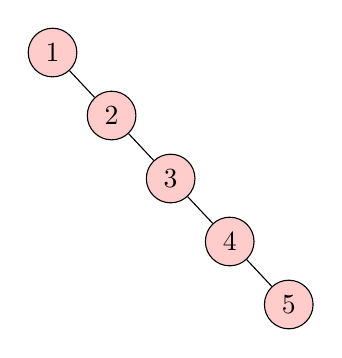
\begin{tikzpicture}[
          level distance=0.8cm,
          every node/.style={circle, draw, minimum size=0.6cm, fill=red!20}
        ]
          \node {1}
            child[missing] {}
            child {node {2}
              child[missing] {}
              child {node {3}
                child[missing] {}
                child {node {4}
                  child[missing] {}
                  child {node {5}}
                }
              }
            };
        \end{tikzpicture}
      \end{center}
      Height = n

      Operations: O(n)
    \end{column}

    \begin{column}{0.5\textwidth}
      \textbf{Balanced BST}
      \begin{center}
        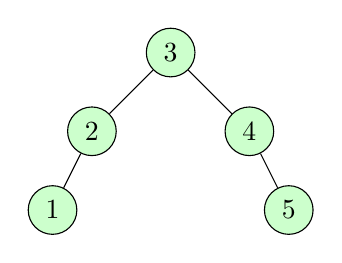
\begin{tikzpicture}[
          level distance=1cm,
          level 1/.style={sibling distance=2cm},
          level 2/.style={sibling distance=1cm},
          every node/.style={circle, draw, minimum size=0.6cm, fill=green!20}
        ]
          \node {3}
            child {node {2}
              child {node {1}}
              child[missing] {}
            }
            child {node {4}
              child[missing] {}
              child {node {5}}
            };
        \end{tikzpicture}
      \end{center}
      Height = log n

      Operations: O(log n)
    \end{column}
  \end{columns}

  \vspace{0.3cm}
  \textbf{Solution:} Self-balancing trees (AVL, Red-Black)
\end{frame}

\begin{frame}{AVL Trees}
  \textbf{Definition:} BST where height difference of left and right subtrees $\leq$ 1 for all nodes.

  \vspace{0.3cm}
  \textbf{Balance Factor:} height(left) - height(right)
  \begin{itemize}
    \item Must be -1, 0, or +1 for all nodes
  \end{itemize}

  \vspace{0.3cm}
  \begin{center}
    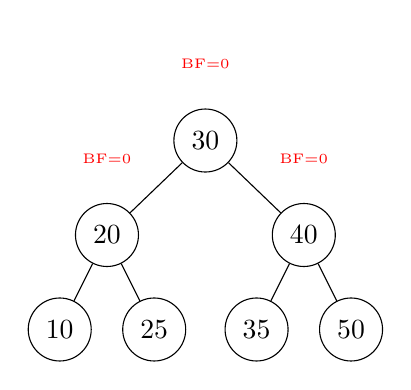
\begin{tikzpicture}[
      level distance=1.2cm,
      level 1/.style={sibling distance=2.5cm},
      level 2/.style={sibling distance=1.2cm},
      every node/.style={circle, draw, minimum size=0.8cm}
    ]
      \node (avl30) {30}
        child {node (avl20) {20}
          child {node {10}}
          child {node {25}}
        }
        child {node (avl40) {40}
          child {node {35}}
          child {node {50}}
        };

      \node[above=0.1cm of avl30, draw=none, red] {\tiny BF=0};
      \node[above=0.1cm of avl20, draw=none, red] {\tiny BF=0};
      \node[above=0.1cm of avl40, draw=none, red] {\tiny BF=0};
    \end{tikzpicture}
  \end{center}

  \textbf{Properties:}
  \begin{itemize}
    \item Height is always O(log n)
    \item All operations O(log n)
    \item More rotations than Red-Black trees
  \end{itemize}
\end{frame}

\begin{frame}{AVL Tree Rotations}
  \textbf{Four Rotation Cases:}

  \vspace{0.3cm}
  \begin{columns}[T]
    \begin{column}{0.5\textwidth}
      \textbf{1. Left-Left (LL)}

      Single right rotation

      \vspace{0.2cm}
      \begin{center}
        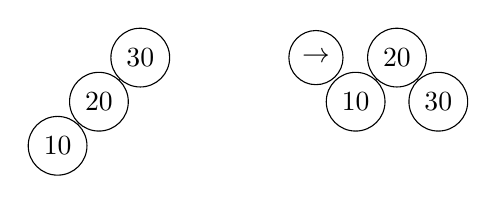
\begin{tikzpicture}[
          level distance=0.8cm,
          level 1/.style={sibling distance=1.5cm},
          every node/.style={circle, draw, minimum size=0.5cm},
          scale=0.7
        ]
          \node (ll30) {30}
            child {node {20}
              child {node {10}}
              child[missing] {}
            }
            child[missing] {};

          \node[right=1.5cm of ll30] {$\rightarrow$};

          \node[right=2.5cm of ll30] {20}
            child {node {10}}
            child {node {30}};
        \end{tikzpicture}
      \end{center}

      \textbf{3. Left-Right (LR)}

      Left rotate, then right rotate
    \end{column}

    \begin{column}{0.5\textwidth}
      \textbf{2. Right-Right (RR)}

      Single left rotation

      \vspace{0.2cm}
      \begin{center}
        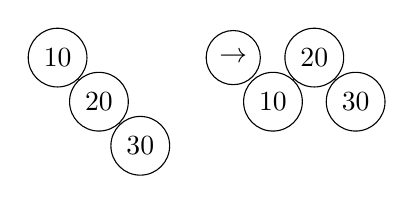
\begin{tikzpicture}[
          level distance=0.8cm,
          level 1/.style={sibling distance=1.5cm},
          every node/.style={circle, draw, minimum size=0.5cm},
          scale=0.7
        ]
          \node (rr10) {10}
            child[missing] {}
            child {node {20}
              child[missing] {}
              child {node {30}}
            };

          \node[right=1.5cm of rr10] {$\rightarrow$};

          \node[right=2.5cm of rr10] {20}
            child {node {10}}
            child {node {30}};
        \end{tikzpicture}
      \end{center}

      \textbf{4. Right-Left (RL)}

      Right rotate, then left rotate
    \end{column}
  \end{columns}
\end{frame}

\begin{frame}[fragile]{AVL Tree Rotation Implementation}
  \begin{lstlisting}[language=Python, basicstyle=\ttfamily\footnotesize]
def _rotate_right(self, y):
    """Right rotation"""
    x = y.left
    T2 = x.right

    x.right = y
    y.left = T2

    y.height = 1 + max(self._get_height(y.left),
                       self._get_height(y.right))
    x.height = 1 + max(self._get_height(x.left),
                       self._get_height(x.right))
    return x

def _rotate_left(self, x):
    """Left rotation"""
    y = x.right
    T2 = y.left

    y.left = x
    x.right = T2

    x.height = 1 + max(self._get_height(x.left),
                       self._get_height(x.right))
    y.height = 1 + max(self._get_height(y.left),
                       self._get_height(y.right))
    return y

def _get_balance(self, node):
    if not node:
        return 0
    return self._get_height(node.left) - self._get_height(node.right)
  \end{lstlisting}
\end{frame}

\begin{frame}{Red-Black Trees}
  \textbf{Definition:} BST with additional color property for balancing.

  \vspace{0.3cm}
  \textbf{Properties:}
  \begin{enumerate}
    \item Every node is either red or black
    \item Root is always black
    \item All leaves (NIL) are black
    \item Red nodes have black children (no two red nodes in a row)
    \item All paths from root to leaves have same number of black nodes
  \end{enumerate}

  \vspace{0.3cm}
  \begin{center}
    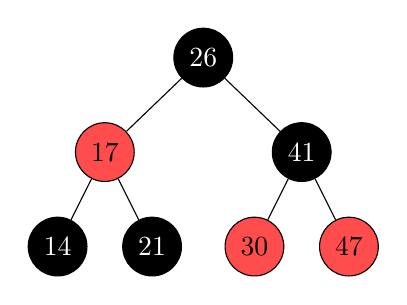
\begin{tikzpicture}[
      level distance=1.2cm,
      level 1/.style={sibling distance=2.5cm},
      level 2/.style={sibling distance=1.2cm},
      every node/.style={circle, draw, minimum size=0.7cm}
    ]
      \node[fill=black, text=white] {26}
        child {node[fill=red!70] {17}
          child {node[fill=black, text=white] {14}}
          child {node[fill=black, text=white] {21}}
        }
        child {node[fill=black, text=white] {41}
          child {node[fill=red!70] {30}}
          child {node[fill=red!70] {47}}
        };
    \end{tikzpicture}
  \end{center}
\end{frame}

\begin{frame}{Red-Black Trees vs AVL Trees}
  \begin{table}
    \centering
    \begin{tabular}{|l|c|c|}
      \hline
      \textbf{Feature} & \textbf{AVL Tree} & \textbf{Red-Black Tree} \\
      \hline
      Balance & Strictly balanced & Approximately balanced \\
      \hline
      Height & $\leq 1.44 \log n$ & $\leq 2 \log n$ \\
      \hline
      Search & Faster & Slightly slower \\
      \hline
      Insert/Delete & More rotations & Fewer rotations \\
      \hline
      Use case & Read-heavy & Insert/delete-heavy \\
      \hline
      Examples & Databases & Java TreeMap, C++ map \\
      \hline
    \end{tabular}
  \end{table}

  \vspace{0.5cm}
  \textbf{Key Takeaway:}
  \begin{itemize}
    \item AVL: Better for lookup-intensive applications
    \item Red-Black: Better for applications with frequent insertions/deletions
  \end{itemize}
\end{frame}

\section{Real-World Applications}

\begin{frame}{Database Indexing}
  \textbf{B-Trees and B+ Trees:} Variants of balanced trees used in databases.

  \vspace{0.3cm}
  \textbf{Why Trees for Databases?}
  \begin{itemize}
    \item Fast search: O(log n)
    \item Efficient range queries
    \item Good disk I/O performance (nodes = disk blocks)
    \item Support for ordered traversal
  \end{itemize}

  \vspace{0.3cm}
  \textbf{B+ Tree Features:}
  \begin{itemize}
    \item All data in leaf nodes
    \item Internal nodes only store keys
    \item Leaves linked for sequential access
    \item Used in: MySQL, PostgreSQL, SQLite
  \end{itemize}

  \vspace{0.3cm}
  \textbf{Example:}
  \begin{itemize}
    \item Index on employee ID
    \item Fast lookups: SELECT * WHERE id = 12345
    \item Range queries: SELECT * WHERE id BETWEEN 1000 AND 2000
  \end{itemize}
\end{frame}

\begin{frame}{Expression Parsing}
  \textbf{Syntax Trees:} Represent mathematical or code expressions.

  \vspace{0.3cm}
  \textbf{Example:} $(3 + 5) \times 2$

  \begin{center}
    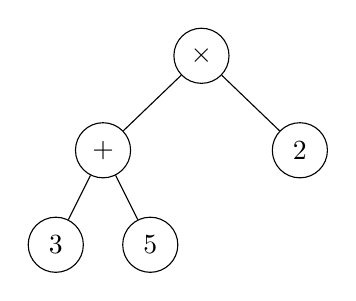
\begin{tikzpicture}[
      level distance=1.2cm,
      level 1/.style={sibling distance=2.5cm},
      level 2/.style={sibling distance=1.2cm},
      every node/.style={circle, draw, minimum size=0.7cm}
    ]
      \node {$\times$}
        child {node {+}
          child {node {3}}
          child {node {5}}
        }
        child {node {2}};
    \end{tikzpicture}
  \end{center}

  \vspace{0.3cm}
  \textbf{Evaluation:}
  \begin{itemize}
    \item Postorder traversal: 3, 5, +, 2, $\times$
    \item Result: $(3 + 5) = 8$, then $8 \times 2 = 16$
  \end{itemize}

  \vspace{0.3cm}
  \textbf{Applications:}
  \begin{itemize}
    \item Compilers and interpreters
    \item Calculators
    \item Abstract Syntax Trees (AST) in programming languages
  \end{itemize}
\end{frame}

\begin{frame}{File Systems}
  \textbf{Directory Structure:} Trees represent hierarchical file organization.

  \vspace{0.3cm}
  \begin{center}
    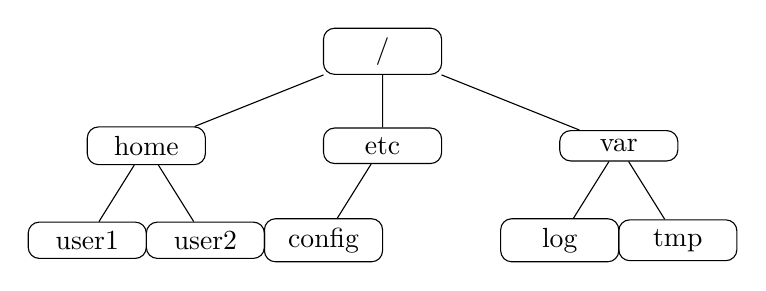
\begin{tikzpicture}[
      level distance=1.2cm,
      level 1/.style={sibling distance=3cm},
      level 2/.style={sibling distance=1.5cm},
      every node/.style={rectangle, draw, rounded corners, minimum width=1.5cm}
    ]
      \node {/}
        child {node {home}
          child {node {user1}}
          child {node {user2}}
        }
        child {node {etc}
          child {node {config}}
          child[missing] {}
        }
        child {node {var}
          child {node {log}}
          child {node {tmp}}
        };
    \end{tikzpicture}
  \end{center}

  \vspace{0.3cm}
  \textbf{Operations:}
  \begin{itemize}
    \item Navigate directories: O(depth)
    \item List contents: Visit children
    \item Calculate directory size: Postorder traversal
    \item Search for files: DFS or BFS
  \end{itemize}
\end{frame}

\begin{frame}{Decision Trees (Machine Learning)}
  \textbf{Decision Trees:} Tree-based models for classification and regression.

  \vspace{0.3cm}
  \begin{center}
    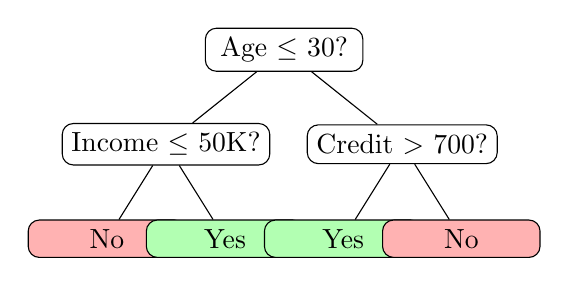
\begin{tikzpicture}[
      level distance=1.2cm,
      level 1/.style={sibling distance=3cm},
      level 2/.style={sibling distance=1.5cm},
      every node/.style={rectangle, draw, rounded corners, minimum width=2cm, align=center}
    ]
      \node {Age $\leq$ 30?}
        child {node {Income $\leq$ 50K?}
          child {node[fill=red!30] {No}}
          child {node[fill=green!30] {Yes}}
        }
        child {node {Credit $>$ 700?}
          child {node[fill=green!30] {Yes}}
          child {node[fill=red!30] {No}}
        };
    \end{tikzpicture}
  \end{center}

  \vspace{0.3cm}
  \textbf{Properties:}
  \begin{itemize}
    \item Internal nodes: Decision rules
    \item Leaves: Predictions (class labels or values)
    \item Path from root to leaf: Decision path
  \end{itemize}

  \vspace{0.3cm}
  \textbf{Algorithms:} ID3, C4.5, CART, Random Forests, Gradient Boosting
\end{frame}

\begin{frame}{Huffman Coding (Compression)}
  \textbf{Huffman Tree:} Optimal prefix-free binary code for data compression.

  \vspace{0.3cm}
  \textbf{Example:} Compress "AAABBC"

  \begin{center}
    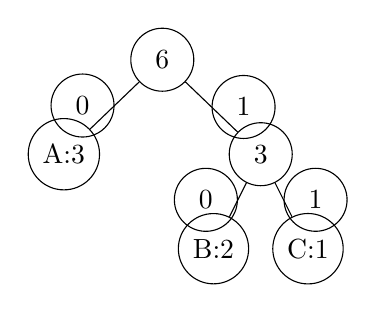
\begin{tikzpicture}[
      level distance=1.2cm,
      level 1/.style={sibling distance=2.5cm},
      level 2/.style={sibling distance=1.2cm},
      every node/.style={circle, draw, minimum size=0.8cm}
    ]
      \node {6}
        child {node {A:3}
          edge from parent node[left] {0}
        }
        child {node {3}
          child {node {B:2}
            edge from parent node[left] {0}
          }
          child {node {C:1}
            edge from parent node[right] {1}
          }
          edge from parent node[right] {1}
        };
    \end{tikzpicture}
  \end{center}

  \vspace{0.3cm}
  \textbf{Encoding:}
  \begin{itemize}
    \item A: 0, B: 10, C: 11
    \item "AAABBC" $\rightarrow$ 0 0 0 10 10 11 (10 bits vs 18 bits)
  \end{itemize}

  \vspace{0.3cm}
  \textbf{Used in:} ZIP, JPEG, MP3
\end{frame}

\section{Complexity Analysis}

\begin{frame}{Tree Operations Complexity}
  \begin{table}
    \centering
    \begin{tabular}{|l|c|c|c|}
      \hline
      \textbf{Operation} & \textbf{BST (avg)} & \textbf{BST (worst)} & \textbf{Balanced} \\
      \hline
      Search & O(log n) & O(n) & O(log n) \\
      \hline
      Insert & O(log n) & O(n) & O(log n) \\
      \hline
      Delete & O(log n) & O(n) & O(log n) \\
      \hline
      Find Min/Max & O(log n) & O(n) & O(log n) \\
      \hline
      Traversal & O(n) & O(n) & O(n) \\
      \hline
    \end{tabular}
  \end{table}

  \vspace{0.5cm}
  \textbf{Key Points:}
  \begin{itemize}
    \item Unbalanced BST: Worst case O(n) when tree becomes skewed
    \item Balanced trees (AVL, Red-Black): Guaranteed O(log n)
    \item Traversals always O(n) - must visit every node
  \end{itemize}
\end{frame}

\begin{frame}{Heap Operations Complexity}
  \begin{table}
    \centering
    \begin{tabular}{|l|c|}
      \hline
      \textbf{Operation} & \textbf{Time Complexity} \\
      \hline
      Insert & O(log n) \\
      \hline
      Extract Max/Min & O(log n) \\
      \hline
      Get Max/Min (peek) & O(1) \\
      \hline
      Build Heap & O(n) \\
      \hline
      Heapify & O(log n) \\
      \hline
      Heap Sort & O(n log n) \\
      \hline
    \end{tabular}
  \end{table}

  \vspace{0.5cm}
  \textbf{Space Complexity:} O(n)

  \vspace{0.3cm}
  \textbf{Note:}
  \begin{itemize}
    \item Get max/min is O(1) - root element
    \item Build heap from array is O(n), not O(n log n)
  \end{itemize}
\end{frame}

\begin{frame}{Space Complexity}
  \textbf{Tree Storage:}

  \vspace{0.3cm}
  \begin{table}
    \centering
    \begin{tabular}{|l|c|}
      \hline
      \textbf{Structure} & \textbf{Space} \\
      \hline
      Binary Tree (pointer-based) & O(n) \\
      \hline
      Complete Binary Tree (array) & O(n) \\
      \hline
      AVL Tree (with height) & O(n) \\
      \hline
      Red-Black Tree (with color) & O(n) \\
      \hline
      Heap (array-based) & O(n) \\
      \hline
    \end{tabular}
  \end{table}

  \vspace{0.3cm}
  \textbf{Additional Space:}
  \begin{itemize}
    \item Recursive traversals: O(h) stack space
    \item Iterative traversals with stack/queue: O(h) or O(w)
      \begin{itemize}
        \item h = height, w = maximum width
      \end{itemize}
    \item Level-order traversal: O(w) for queue
  \end{itemize}
\end{frame}

\section{Summary}

\begin{frame}{Key Concepts Recap}
  \textbf{Binary Trees:}
  \begin{itemize}
    \item Hierarchical structure with at most 2 children per node
    \item Types: Full, Complete, Perfect, Balanced, Skewed
  \end{itemize}

  \vspace{0.3cm}
  \textbf{Binary Search Trees:}
  \begin{itemize}
    \item Ordered binary tree: left $<$ root $<$ right
    \item Operations: Search, Insert, Delete - O(h)
    \item Can degenerate to O(n) without balancing
  \end{itemize}

  \vspace{0.3cm}
  \textbf{Traversals:}
  \begin{itemize}
    \item Inorder (sorted), Preorder (copy), Postorder (delete), Level-order
  \end{itemize}

  \vspace{0.3cm}
  \textbf{Heaps:}
  \begin{itemize}
    \item Complete binary tree with heap property
    \item Priority queue, Heap sort, Top-K problems
  \end{itemize}
\end{frame}

\begin{frame}{Key Concepts Recap (continued)}
  \textbf{Balanced Trees:}
  \begin{itemize}
    \item AVL: Strict balance, faster search
    \item Red-Black: Approximate balance, faster insert/delete
    \item Both guarantee O(log n) operations
  \end{itemize}

  \vspace{0.3cm}
  \textbf{Applications:}
  \begin{itemize}
    \item Database indexing (B-trees, B+ trees)
    \item Expression parsing (syntax trees)
    \item File systems (directory trees)
    \item Machine learning (decision trees)
    \item Compression (Huffman coding)
  \end{itemize}

  \vspace{0.3cm}
  \textbf{Complexity:}
  \begin{itemize}
    \item Balanced trees: O(log n) for search, insert, delete
    \item Heaps: O(log n) for insert/extract, O(1) for peek
    \item Traversals: Always O(n)
  \end{itemize}
\end{frame}

\begin{frame}{When to Use Which Tree?}
  \begin{table}
    \centering
    \small
    \begin{tabular}{|l|l|}
      \hline
      \textbf{Use Case} & \textbf{Tree Type} \\
      \hline
      Fast search in sorted data & BST, AVL, Red-Black \\
      \hline
      Priority queue & Min/Max Heap \\
      \hline
      Frequent inserts/deletes & Red-Black Tree \\
      \hline
      Lookup-heavy workload & AVL Tree \\
      \hline
      Database indexing & B-Tree, B+ Tree \\
      \hline
      Expression evaluation & Syntax Tree \\
      \hline
      File system & N-ary Tree \\
      \hline
      Decision making & Decision Tree \\
      \hline
      Compression & Huffman Tree \\
      \hline
      Range queries & Segment Tree, Interval Tree \\
      \hline
    \end{tabular}
  \end{table}
\end{frame}

\begin{frame}{Practice Problems}
  \textbf{Basic:}
  \begin{itemize}
    \item Implement inorder, preorder, postorder traversals
    \item Find height of a binary tree
    \item Check if a binary tree is a valid BST
    \item Find lowest common ancestor (LCA)
  \end{itemize}

  \vspace{0.3cm}
  \textbf{Intermediate:}
  \begin{itemize}
    \item Serialize and deserialize a binary tree
    \item Convert sorted array to balanced BST
    \item Implement AVL tree with rotations
    \item Find kth smallest element in BST
  \end{itemize}

  \vspace{0.3cm}
  \textbf{Advanced:}
  \begin{itemize}
    \item Implement Red-Black tree
    \item Morris traversal (constant space)
    \item Segment tree for range queries
    \item Trie for prefix matching
  \end{itemize}
\end{frame}

\begin{frame}{Next Steps}
  \textbf{Continue Learning:}
  \begin{itemize}
    \item Advanced trees: Trie, Segment Tree, Fenwick Tree
    \item Graph algorithms (trees are special graphs)
    \item Dynamic programming with trees
    \item Practice on LeetCode, HackerRank
  \end{itemize}

  \vspace{0.3cm}
  \textbf{Resources:}
  \begin{itemize}
    \item CLRS: Introduction to Algorithms
    \item GeeksforGeeks tree tutorials
    \item Visualgo.net for visualizations
    \item Project: Implement your own balanced tree library
  \end{itemize}

  \vspace{0.3cm}
  \textbf{Real-World Projects:}
  \begin{itemize}
    \item Build a simple database with B-tree indexing
    \item Create an expression evaluator
    \item Implement file compression with Huffman coding
    \item Design a decision tree classifier
  \end{itemize}
\end{frame}

\begin{frame}
  \begin{center}
    {\Huge Thank You!}

    \vspace{1cm}
    {\Large Questions?}

    \vspace{1cm}
    \textbf{Trees: The Foundation of Hierarchical Thinking}
  \end{center}
\end{frame}

\end{document}
